\subsection{Integer}

\begin{frame}
    \frametitle{Unary}
    Number of consecutive 1 bits with 0 as the last bit
    \begin{equation}
        \begin{aligned}
            &\text{Binary}\textsubscript{x}=\textcolor{black}{b\textsubscript{n-1}b\textsubscript{n-2}...b\textsubscript{1}b\textsubscript{0}}\\
            &b\textsubscript{i}=
                \begin{cases}
                    1,& \text{if } x\geq i+1\\
                    0, & \text{otherwise}
                \end{cases}
        \end{aligned}
    \end{equation}
\end{frame}


\begin{frame}
    \frametitle{Binary}
    The number representation in base 2
    \begin{equation}
        \begin{aligned}
            &\text{Binary}\textsubscript{x}=\textcolor{black}{b\textsubscript{n-1}b\textsubscript{n-2}...b\textsubscript{1}b\textsubscript{0}}\\
            &x=\sum_{i=0}^{n-1} b_i \times 2^i
        \end{aligned}
    \end{equation}
\end{frame}

\begin{frame}
    \frametitle{Sign magnitude}
    The binary number representation system with a sign bit
    \begin{equation}
        \begin{aligned}
            &\text{Binary}\textsubscript{x}=\textcolor{red}{s}\textcolor{black}{b\textsubscript{n-2}b\textsubscript{n-3}...b\textsubscript{1}b\textsubscript{0}}\\
            &x=(-1)^{\textcolor{red}{s}} \times \sum_{i=0}^{n-2} b_i \times 2^i
        \end{aligned}
    \end{equation}
\end{frame}

\begin{frame}
    \frametitle{One's complement}
    The bynary number representation with one's complement
    \begin{equation}
        \begin{aligned}
            &\text{Binary}\textsubscript{x}=\textcolor{red}{s}\textcolor{black}{b\textsubscript{n-2}b\textsubscript{n-3}...b\textsubscript{1}b\textsubscript{0}}\\
            &x=\begin{cases}
                    \sum_{i=0}^{n-2} b_i \times 2^i,& \text{if \textcolor{red}{sign} positive} \\
                    (-1) \times \sum_{i=0}^{n-2} \overline{b_i} \times 2^i, & \text{otherwise}
            \end{cases} 
        \end{aligned}
    \end{equation}
\end{frame}

\begin{frame}
    \frametitle{Two's complement}
    The binary number representation with two's complement
    \begin{equation}
        \begin{aligned}
            &\text{Binary}\textsubscript{x}=\textcolor{red}{s}\textcolor{black}{b\textsubscript{n-2}b\textsubscript{n-3}...b\textsubscript{1}b\textsubscript{0}}\\
            &x=\begin{cases}
                    \sum_{i=0}^{n-2} b_i \times 2^i,& \text{if \textcolor{red}{sign} positive} \\
                    (-1) \times ((\sum_{i=0}^{n-2} \overline{b_i} \times 2^i) + 1), & \text{otherwise}
            \end{cases} 
        \end{aligned}
    \end{equation}
\end{frame}

\begin{frame}
    \frametitle{Bias}
    The binary number representation with bias
    \begin{equation}
        \begin{aligned}
            &\text{Binary}\textsubscript{x}=\textcolor{black}{b\textsubscript{n-1}b\textsubscript{n-2}...b\textsubscript{1}b\textsubscript{0}}\\
            &\text{Bias}=2^{n-1}-1\\
            &x=(\sum_{i=0}^{n-1} b_i \times 2^i) - \text{Bias}
        \end{aligned}
    \end{equation}
\end{frame}

\begin{frame}
    \frametitle{Unary negative}
    \begin{equation}
        \begin{aligned}
            &\text{Binary}\textsubscript{x}=\textcolor{black}{b\textsubscript{n-1}b\textsubscript{n-2}...b\textsubscript{1}b\textsubscript{0}}\\
            &b\textsubscript{i}=
                \begin{cases}
                    1, & \text{if } (x\geq i \text{ and } x \geq 0)  \text{ or } (|x| \leq i \text{ and } x < 0)\\
                    0,& \text{otherwise}\\
                \end{cases}
        \end{aligned}
    \end{equation}
\end{frame}

\begin{frame}
    \frametitle{Unary}
\end{frame}

\subsection{Fractional}
\begin{frame}
    \frametitle{Fractional}
    Fractional numbers as $Q(ns, ds)$, where $ns$ is the numerator size and $ds$ is the denominator size.
    \begin{equation}
        \begin{aligned}
            &\text{Binary}\textsubscript{x}=\textcolor{red}{s}\textcolor{black}{n\textsubscript{ns-2}n\textsubscript{ns-3}...n\textsubscript{1}n\textsubscript{0}}\textcolor{orange}{d\textsubscript{ds-1}d\textsubscript{ds-2}...d\textsubscript{1}d\textsubscript{0}}\\
            &x=(-1)^{\textcolor{red}{s}} \times \frac{\sum_{i=0}^{ns-2} n_i \times 2^i}{\textcolor{orange}{\sum_{i=0}^{ds-1} d_i \times 2^i}}
        \end{aligned}
    \end{equation}
\end{frame}

\begin{frame}
    \frametitle{Fractional}
\end{frame}

\subsection{Fixed Point}
\begin{frame}
    \frametitle{Fixed Point}
    Fixed point numbers as $FP(is, fs)$, where $is$ is the integer part size and $fs$ is the fractional part size.
    \begin{equation}
        \begin{aligned}
            &\text{Binary}\textsubscript{x}=\textcolor{red}{s}\textcolor{black}{i\textsubscript{is-2}i\textsubscript{is-3}...i\textsubscript{1}i\textsubscript{0}}\textcolor{orange}{f\textsubscript{fs-1}f\textsubscript{fs-2}...f\textsubscript{1}f\textsubscript{0}}\\
            &x=\begin{cases}
                    (\sum_{j=0}^{is-2} i_j \times 2^j) + \textcolor{orange}{(\sum_{j=0}^{fs-1} f_j \times 2^{j-fs})},& \text{if \textcolor{red}{sign} positive} \\
                    (-1) \times ((\sum_{j=0}^{is-2} \overline{i}_j \times 2^j) + \textcolor{orange}{(\sum_{j=0}^{fs-1} \overline{f}_j \times 2^{j-fs})} + \frac{1}{ \textcolor{orange}{2^{fs}}}), & \text{otherwise}
            \end{cases}
        \end{aligned}
    \end{equation}
\end{frame}


\begin{frame}
    \frametitle{Fixed Point}
\end{frame}

\subsection{Floating Point}
\begin{frame}
    \frametitle{Simple Floating Point}
    Simple floating point numbers as $FloatP(es, fs)$, where $es$ is the exponent size and $fs$ is the fractional part size (mantissa).
    $x=(-1)^{\text{sign}} \times 2^{\text{exponent}}  \times 1.f$.
    \begin{equation}
        \begin{aligned}
            \text{Binary}\textsubscript{x}&=\textcolor{red}{s}\textcolor{ForestGreen}{e\textsubscript{es-1}e\textsubscript{es-2}...e\textsubscript{1}e\textsubscript{0}}\textcolor{orange}{m\textsubscript{fs-1}m\textsubscript{fs-2}...m\textsubscript{1}m\textsubscript{0}}\\
            \text{Bias}&=2^{es-1}-1\\
            e&=\textcolor{ForestGreen}{\sum_{i=0}^{es-1} e_i \times 2^{i}} - \text{Bias}\\
            x&=(-1)^{\textcolor{red}{s}} \times \begin{cases}
                    0, \text{if } \forall\ i<es\ e_i=0\ \And \forall\ i<fs\ m_i=0 \\
                    2^e \times (1 + \textcolor{orange}{\frac{\sum_{i=0}^{fs-1} m_i \times 2^i}{2^{fs}}}), \text{otherwise}
            \end{cases}
        \end{aligned}
    \end{equation}
\end{frame}

\begin{frame}
    \frametitle{Simple Floating Point}
\end{frame}

\begin{frame}
    \frametitle{IEEE754 Floating Point}
    Can use the notation $IEEE754(es, fs)$, where $es$ is the exponent size and $fs$ is the fractional part size (mantissa).
\begin{equation}
    \resizebox{0.9\textwidth}{!}{%
    $
    \begin{aligned}
        x&=(-1)^{\textcolor{red}{s}} \times \begin{cases}
                0 &, \text{if } \textcolor{ForestGreen}{\forall\ i<es\ e_i=0}\ \And \textcolor{orange}{\forall\ i<fs\ m_i=0} \\
                2^{\textcolor{ForestGreen}{e}+1} \times \textcolor{orange}{\frac{\sum_{i=0}^{fs-1} m_i \times 2^i}{2^{fs}}} &, \text{if } \textcolor{ForestGreen}{\forall\ i<es\ e_i=0}\ \And \textcolor{orange}{\exists\ i<fs\ m_i\neq0} \\
                \textcolor{Plum}{\infty} &, \text{if } \textcolor{ForestGreen}{\forall\ i<es\ e_i=1}\ \And \textcolor{orange}{\forall\ i<fs\ m_i=0} \\
                 \textcolor{Plum}{sNaN} &, \text{if } \textcolor{ForestGreen}{\forall\ i<es\ e_i=1}\ \And \textcolor{orange}{m_{fs-1}=0} \And \textcolor{orange}{\exists\ i<fs-1\ m_i\neq0} \\
                 \textcolor{Plum}{qNaN} &, \text{if } \textcolor{ForestGreen}{\forall\ i<es\ e_i=1}\ \And \textcolor{orange}{m_{fs-1}=1} \\
                2^{\textcolor{ForestGreen}{e}} \times (1 + \textcolor{orange}{\frac{\sum_{i=0}^{fs-1} m_i \times 2^i}{2^{fs}}}) &, \text{otherwise}
        \end{cases}
    \end{aligned}$%
    }
\end{equation}

\end{frame}

\begin{frame}
    \frametitle{IEEE754 Floating Point}
\end{frame}


\begin{frame}
    \frametitle{Morris Floating Point}
    In the Morris floating point representation we use the following notation $Morris(s, g)$, where $s$ is size and $g$ is the size of the exponent size.
    \begin{equation}
        \resizebox{0.9\textwidth}{!}{%
        $
        \begin{aligned}
            \text{Binary}\textsubscript{x}&=\textcolor{blue}{G\textsubscript{g-1}G\textsubscript{g-2}...G\textsubscript{1}G\textsubscript{0}}\textcolor{red}{s\textsubscript{e}}\textcolor{ForestGreen}{e\textsubscript{es-1}e\textsubscript{es-2}...e\textsubscript{1}e\textsubscript{0}}\textcolor{red}{s\textsubscript{f}}\textcolor{orange}{m\textsubscript{fs-1}m\textsubscript{fs-2}...m\textsubscript{1}m\textsubscript{0}}\\
            G&=\textcolor{blue}{\sum_{i=0}^{g-1} G_i \times 2^{i}}\\
            es&=G+1\\
            e&=(-1)^{\textcolor{red}{s\textsubscript{e}}}\textcolor{ForestGreen}{\sum_{i=0}^{es-1} e_i \times 2^{i}}\\
            x&=(-1)^{\textcolor{red}{s\textsubscript{f}}} \times \begin{cases}
                    0 &, \text{if } \forall\ i\ \textcolor{ForestGreen}{e_i=0}\ \And\ \textcolor{orange}{m_i=0}\ \And\ \textcolor{blue}{G_i=0}\\
                    NR &, \text{all bits $1$}\\
                    2^{\textcolor{ForestGreen}{e}} \times (1 + \textcolor{orange}{\frac{\sum_{i=0}^{fs-1} m_i \times 2^i}{2^{fs}}}) &, \text{otherwise}
            \end{cases}
        \end{aligned}$%
        }
    \end{equation}
    \note{
   The Morris floating point system is given by the size and the size of the exponent size called simple $g$. The first $g$ bits represent the value $G$, which is added with $1$ to obtain the exponent size ($es$). The next bit is the exponent sign bit, followed by $es$ bits, which represent the absolute value of the exponent. The next bit is the fraction sign, and the remaining bits are considered fraction bits. The hidden bit is always $1$. The value is computed by $2^{\text{exponent}} \times (-1)^{\text{fractionSign}} \times (1+\frac{f}{2^{fs}})$, where exponent is $(-1)^{\text{exponentSign}} \times \text{exponentAbsoluteValue}$. The $0$ is represented by all bits of zero, and error cases are represented by only $1s$
    }
\end{frame}


\begin{frame}
    \frametitle{Morris Floating Point}
\end{frame}


\begin{frame}
    \frametitle{Posit}
    $Posit(size, es)$ is given by $size$ and exponent size ($es$).
    \begin{equation}
        \resizebox{0.9\textwidth}{!}{%
        $
        \begin{aligned}
            \text{Binary}\textsubscript{x}&=\textcolor{red}{s}\textcolor{black}{b\textsubscript{size-2}b\textsubscript{size-3}...b\textsubscript{1}b\textsubscript{0}}\\
            \text{AbsoluteBits}\textsubscript{x}&=\begin{cases}
                \overline{\text{Binary}\textsubscript{x}} + 1 &, \text{if \textcolor{red}{sign} negative}\\
                 \text{Binary}\textsubscript{x} &, \text{otherwise}
            \end{cases}\\
            \text{AbsoluteBits}\textsubscript{x}&=\textcolor{red}{0}\textcolor{blue}{r\textsubscript{0}r\textsubscript{1}...r\textsubscript{rs-2}\overline{r\textsubscript{rs-1}}}\textcolor{ForestGreen}{e\textsubscript{es-1}e\textsubscript{es-2}...e\textsubscript{1}e\textsubscript{0}}\textcolor{orange}{m\textsubscript{fs-1}m\textsubscript{fs-2}...m\textsubscript{1}m\textsubscript{0}}\\
            k&=\begin{cases}
                \textcolor{blue}{rs}-2 &, \text{if } \textcolor{blue}{r_0=1}\\
                -(\textcolor{blue}{rs}-1) &, \text{otherwise}
            \end{cases}\\
            e&=\textcolor{blue}{k} \times 2^{es} + \textcolor{ForestGreen}{\sum_{i=0}^{es-1} e_i \times 2^{i}}\\
            x&=(-1)^{\textcolor{red}{s}} \times \begin{cases}
                    0 &, \text{all bits of \text{Binary}\textsubscript{x} $0$}\\
                    NaR &, \text{first bit $1$ and the rest $0$ for \text{Binary}\textsubscript{x}}\\
                    2^{\textcolor{ForestGreen}{e}} \times (1 + \textcolor{orange}{\frac{\sum_{i=0}^{fs-1} m_i \times 2^i}{2^{fs}}}) &, \text{otherwise}
            \end{cases}
        \end{aligned}$%
        }
    \end{equation}
\end{frame}


\begin{frame}
    \frametitle{Posit}
\end{frame}

\begin{frame}
    \frametitle{Until now}
    \begin{table}[ht]
        %\begin{center}
        \resizebox{0.65\columnwidth}{!}{%
        \begin{tabular}{|p{1em}|p{5.7em}|p{3.4em}|p{16em}|c|c|c|c|}
            \hline
            \multirow{2}{*}{Set} & \multirow{2}{*}{NRS} & \multirow{2}{*}{Precision} & \multirow{2}{*}{m-layer} &  \multirow{2}{*}{$[x]$} & \multicolumn{3}{|c|}{s-layer given  h-layer} \\
            \cline{6-8}
            &&&&&5&-5&1.25\\
            \hline
            % N natural numbers set
            %\iffalse
            \multirow{4}{*}{$\mathbb{N}$} & \multirow{2}{*}{Unary} & IP & $\mathbb{N}$ & & 11111 & NR & NR\\
            \cline{3-8}
            & & VP/FP& $\{x, x \in \mathbb{N} , x < n \}$ & $U[8,r]$ & 00011111 & NR & NR\\
            \cline{2-8}
            & \multirow{2}{*}{Base 2} & IP & $\mathbb{N}$ & & 101 & NR & NR\\
            \cline{3-8}
            & & VP/FP & $\{x, x \in \mathbb{N} , x < 2^n \}$ & $\mathbb{N}[8,r]$ & 00000101 & NR & NR\\
            \hline
            % Z integer numbers set
            \multirow{8}{*}{$\mathbb{Z}$} & \multirow{2}{*}{Sign} & IP & $\mathbb{Z}$ & & \textcolor{red}{0}101 & \textcolor{red}{1}101 & NR\\
            \cline{3-8}
            & & VP/FP & $\{(s,x), s \in \{0,1\}, x \in \mathbb{N}[n-1, r] \}$ & $\mathbb{Z}[8,r]$ & \textcolor{red}{0}0000101 & \textcolor{red}{1}0000101 & NR\\
            \cline{2-8}
            & \multirow{2}{*}{1'complement} & IP & $\mathbb{Z}$ & & \textcolor{red}{0}101 & \textcolor{red}{1}010 & NR\\
            \cline{3-8}
            & & VP/FP & $\{x, x \in \mathbb{Z} , |x| < 2^n \}$ & [8,r] & \textcolor{red}{0}0000101 & \textcolor{red}{1}1111010 & NR\\
            \cline{2-8}
            & \multirow{2}{*}{2'complement} & IP & $\mathbb{Z}$ & & \textcolor{red}{0}101 & \textcolor{red}{1}011 & NR\\
            \cline{3-8}
            & & VP/FP & $\{x, x \in \mathbb{Z} , -2^{n-1} \leq x < 2^{n-1} \}$ & [8,r] & \textcolor{red}{0}0000101 & \textcolor{red}{1}1111011 & NR\\
            \cline{2-8}
            &\multirow{2}{*}{Bias} & IP & $\{y-bias, y \in \mathbb{N}\}$ & [10] & 1111 & 0101 & NR\\
            \cline{3-8}
            & & VP/FP & $\{y-bias, y \in \mathbb{N}[n, r]\}$ & $\text{Bias}[10,8,r]$ & 00001111 & 00000101 & NR\\
            \hline
            % Q rational numbers set
            \multirow{12}{*}{$\mathbb{Q}$} & \multirow{2}{*}{Fractional} & IP & $\mathbb{Q}$ & & \textcolor{red}{0}101/1 & \textcolor{red}{1}101/1 & \textcolor{red}{0}101/100\\
            \cline{3-8}
            & & VP/FP & $\{\frac{x}{y}, x \in \mathbb{Z}[ns, r], y \in \mathbb{N}[ds, r]  \}$ & $\mathbb{Q}[4,3,r]$ & \textcolor{red}{0}101\textcolor{orange}{001} & \textcolor{red}{1}101\textcolor{orange}{001} & \textcolor{red}{0}101\textcolor{orange}{100}\\
            \cline{2-8}
            %FixedPoint
            & \multirow{2}{*}{Fixed Point} & IP & $\{\frac{x}{2^y}, x \in \mathbb{Z}, y \in \mathbb{N}  \}$ & & \textcolor{red}{0}101\textcolor{blue}{.}0 & \textcolor{red}{1}101\textcolor{blue}{.}0 & \textcolor{red}{0}001\textcolor{blue}{.}10\\
            \cline{3-8}
            & & VP/FP & $\{\frac{x}{2^{bp}}, x \in \mathbb{Z}[is+fs, r]  \}$ & $\text{FixedPoint}[4,3,r]$ & \textcolor{red}{0}101\textcolor{blue}{.}\textcolor{orange}{000} & \textcolor{red}{1}101\textcolor{blue}{.}\textcolor{orange}{000} & \textcolor{red}{0}001\textcolor{blue}{.}\textcolor{orange}{100}\\
            \cline{2-8}
            % Floating Point
            & \multirow{2}{*}{Floating Point} & IP & $\{x \times 2^y, x \in [1,2), y \in \mathbb{Z}  \}$ & $\text{FloatingPoint}[\infty]$ & \textcolor{red}{0}1\textcolor{blue}{.}\textcolor{orange}{010}/\textcolor{red}{0}\textcolor{ForestGreen}{10} & \textcolor{red}{1}1\textcolor{blue}{.}\textcolor{orange}{010}/\textcolor{red}{0}\textcolor{ForestGreen}{10} & \textcolor{red}{0}1\textcolor{blue}{.}\textcolor{orange}{100}/\textcolor{red}{0}\textcolor{ForestGreen}{0}\\
            \cline{3-8}
            & & VP/FP & $\{(1 + \frac{f}{2^{fs}}) \times 2^{exp}, (f,exp) \in M, M = ((\mathbb{N}[fs, r] \times \text{Bias}[es, 2^{es-1}-1, r]) \setminus \{(0, -2^{es-1}+1)\})  \} \cup \{0\}$ & \text{FloatingPoint}[4,3,r] & \textcolor{red}{0}\textcolor{ForestGreen}{1001}\textcolor{orange}{010} & \textcolor{red}{1}\textcolor{ForestGreen}{1001}\textcolor{orange}{010} & \textcolor{red}{0}\textcolor{ForestGreen}{0111}\textcolor{orange}{100}\\
            \cline{2-8}
            %IEEE754
            & \multirow{2}{*}{IEEE754} & IP & $\text{FloatingPoint}[\infty]$ & & \textcolor{red}{0}1\textcolor{blue}{.}\textcolor{orange}{010}/\textcolor{red}{0}\textcolor{ForestGreen}{10} & \textcolor{red}{1}1\textcolor{blue}{.}\textcolor{orange}{010}/\textcolor{red}{0}\textcolor{ForestGreen}{10} & \textcolor{red}{0}1\textcolor{blue}{.}\textcolor{orange}{100}/\textcolor{red}{0}\textcolor{ForestGreen}{0}\\
            \cline{3-8}
            & & VP/FP & $\{(1 + \frac{f}{2^{fs}}) \times 2^{exp}, x \in \mathbb{N}[fs, r], exp \in \text{Bias}[es, 2^{es-1}-1, r] \setminus \{-2^{es-1}+1, 2^{es-1}\})  \} \cup \{ \frac{x}{2^{fs}} \times 2^{exp}, f \in (\mathbb{N}[fs, r] \setminus \{0\}), exp = -2^{es-1}+2 \}  \} \cup \{0\}$ & $\text{IEEE754}[4,3,r]$ & \textcolor{red}{0}\textcolor{ForestGreen}{1001}\textcolor{orange}{010} & \textcolor{red}{1}\textcolor{ForestGreen}{1001}\textcolor{orange}{010} & \textcolor{red}{0}\textcolor{ForestGreen}{0111}\textcolor{orange}{100}\\
            \cline{2-8}
            %Morris
            & \multirow{2}{*}{Morris} & IP & $\text{FloatingPoint}[\infty]$ & & \textcolor{red}{0}1\textcolor{blue}{.}\textcolor{orange}{010}/\textcolor{red}{0}\textcolor{ForestGreen}{10} & \textcolor{red}{1}1\textcolor{blue}{.}\textcolor{orange}{010}/\textcolor{red}{0}\textcolor{ForestGreen}{10} & \textcolor{red}{0}1\textcolor{blue}{.}\textcolor{orange}{100}/\textcolor{red}{0}\textcolor{ForestGreen}{0}\\
            \cline{3-8}
            & & VP/FP & $\{0\} \cup \bigcup_{G \in \mathbb{N}[g, r]} A_G=\{(-1)^{sign \times p} \times (1 + \frac{f}{2^{fs}}) \times 2^{exp}, es = min(G+1,n-g-1), t = max(G+1-(n-g-1), 0), e \in \mathbb{Z}[es+1,r], exp=e \times 2^t, fs=max(n-2-es-g,0), p=max(n-g-1-es-fs,0), sign \in \{0,1\}, f \in \mathbb{N}[fs, r] \}$ & $\text{Morris}[8,2,r]$ & \textcolor{blue}{01}\textcolor{red}{0}\textcolor{ForestGreen}{10}\textcolor{red}{0}\textcolor{orange}{01}&\textcolor{blue}{01}\textcolor{red}{0}\textcolor{ForestGreen}{10}\textcolor{red}{1}\textcolor{orange}{01}&\textcolor{blue}{00}\textcolor{red}{0}\textcolor{ForestGreen}{0}\textcolor{red}{0}\textcolor{orange}{010}\\
            \cline{2-8}
            %Posit
            & \multirow{2}{*}{Posit} & IP & $\text{FloatingPoint}[\infty]$ & & \textcolor{red}{0}1\textcolor{blue}{.}\textcolor{orange}{010}/\textcolor{red}{0}\textcolor{ForestGreen}{10} & \textcolor{red}{1}1\textcolor{blue}{.}\textcolor{orange}{010}/\textcolor{red}{0}\textcolor{ForestGreen}{10} & \textcolor{red}{0}1\textcolor{blue}{.}\textcolor{orange}{100}/\textcolor{red}{0}\textcolor{ForestGreen}{0}\\
            \cline{3-8}
            & & VP/FP & $\{0\} \cup \bigcup_{kl \in \mathbb{N}, 0 < kl \leq n -2 } A_{kl}=\{(-1)^{sign} \times (1 + \frac{f}{2^{fs}}) \times 2^{exp+regime},t=max(0, es-(n-2-kl)), e \in \mathbb{N}[es-t, r], regime \in \{(kl-1) \times 2^{es},-kl \times 2 ^{es}\}, exp = e \times 2^t, fs = max(0, n-2-kl-es), f \in \mathbb{N}[fs, r], sign \in \{0,1\} \}$ & [8,2,r] & \textcolor{red}{0}\textcolor{blue}{10}\textcolor{ForestGreen}{10}\textcolor{orange}{010}&\textcolor{red}{1}0101110 & \textcolor{red}{0}\textcolor{blue}{10}\textcolor{ForestGreen}{00}\textcolor{orange}{100}\\
            \hline
        \end{tabular}%
        }
        %\end{center}
        \label{tabel:nrssback}
        \end{table}
\end{frame}

\begin{frame}
    \frametitle{My proposals}
    \begin{itemize}
        \item Morris Hidden Exponent Bit \begin{equation}
            \textcolor{red}{s_{f}}\textcolor{blue}{G\textsubscript{g-1}G\textsubscript{g-2}...G\textsubscript{0}}\textcolor{red}{s_{e}}\textcolor{brown}{e\textsubscript{es-1}e\textsubscript{es-2}...e\textsubscript{0}}\textcolor{orange}{f\textsubscript{fs-1}f\textsubscript{fs-2}...f\textsubscript{0}}
        \end{equation}
        \item Morris Hidden Exponent Bit with Bias G \begin{equation}
            \textcolor{red}{s}\textcolor{blue}{G\textsubscript{g-1}G\textsubscript{g-2}...G\textsubscript{0}}\textcolor{brown}{e\textsubscript{es-1}e\textsubscript{es-2}...e\textsubscript{0}}\textcolor{orange}{f\textsubscript{fs-1}f\textsubscript{fs-2}...f\textsubscript{0}}
        \end{equation}
        \item Morris Hidden Exponent Bit with Unary G \begin{equation}
            \textcolor{red}{s}\textcolor{blue}{r\textsubscript{0}r\textsubscript{1}...r\textsubscript{rs-2}\overline{r\textsubscript{rs-1}}}\textcolor{brown}{e\textsubscript{es-1}e\textsubscript{es-2}...e\textsubscript{0}}\textcolor{orange}{f\textsubscript{fs-1}f\textsubscript{fs-2}...f\textsubscript{0}}
        \end{equation}
    \end{itemize}
\end{frame}


\begin{frame}
    \frametitle{Morris Hidden Exponent Bit}
The major problem of Morris floating numbers is the multiple ways of representing the same number.
A solution for this is in borrowing the concept of hidden bit from mantissa.
The $g$ field not only represents the $G$ value which dictates the exponent size but also the position of the most significant bit set in the exponent.
If the value of the exponent size is kept as $G+1$, then the minimum absolute value of the exponent is 2 when $G=0$.
\end{frame}
\begin{frame}
    \frametitle{Morris Hidden Exponent Bit}

    $es=G-1$\\
\begin{equation}
    \text{exponent} = \begin{cases}
    (-1)^{\text{exponent sign}} \times ( 2^{es} + \text{binaryExponent} ), & es \neq -1\\
    0, & es=-1.
\end{cases}
\end{equation}
\begin{equation}
    \text{value} = \begin{cases}
    0, & \text{all bits 0}\\
    \text{NR}, & \text{first bit 1 and the rest 0s} \\
    (-1)^{\text{sign}} \times 2^{\text{exponent}} \times (1 + \frac{\text{f}}{2^{\text{fs}}}), & \text{otherwise} \\
  \end{cases}
\end{equation}
\end{frame}

\begin{frame}
    \frametitle{Morris Hidden Exponent Bit with Bias G}
One might argue that the problem of multiple representations is still not solved because even the
exponent may have multiple values (for $es=-1$ the exponent sign does not matter).
The problem stems from having a bit dedicated to the exponent sign.
This is already solved in IEEE754 by using a bias value. A bias value $g$ is proposed.
The exponent sign is the sign of $G$ and the exponent size is $es=|G|-1$.
Another issue with Morris and MorrisHEB representations is that they do not have an order in binary form.
A solution for this is to have the bits of the exponent negated when $G$ is negative.
This makes it easy to implement a hardware compare unit.

\end{frame}


\begin{frame}
    \frametitle{Morris Hidden Exponent Bit with Bias G}
    $\textit{bias}=2^{g-1}-1$. 
    $G=\textit{binary G} - \textit{bias}$
    $es=|G|-1$
    \begin{equation}
        \text{exponent} = \begin{cases}
        \text{signum(G)} \times ( 2^{es} + \text{binaryExponent} ), & es \neq -1\\
        0, & es=-1.
      \end{cases}
    \end{equation}
\end{frame}

\begin{frame}
    \frametitle{Morris Hidden Exponent Bit with Unary G}
    \begin{equation}
        \text{exponent size} = \begin{cases}
        -k - 1, & k < 0 \\
        k - 1, & k \ge 0.
      \end{cases}
    \end{equation}
    \begin{equation}
        k = \begin{cases}
        -\text{NoC0}, & r_0=0 \\
        \text{NoC1} - 1, & r_0=1.
      \end{cases}
    \end{equation}
    \begin{equation}
        \text{exponent} = \begin{cases}
        \text{signum(k)} \times ( 2^{es} + \text{binaryExponent} ), & es \neq -1\\
        0, & es=-1.
      \end{cases}
    \end{equation}
\end{frame}

\begin{frame}
    \frametitle{Addition}

\begin{figure}[tp]
    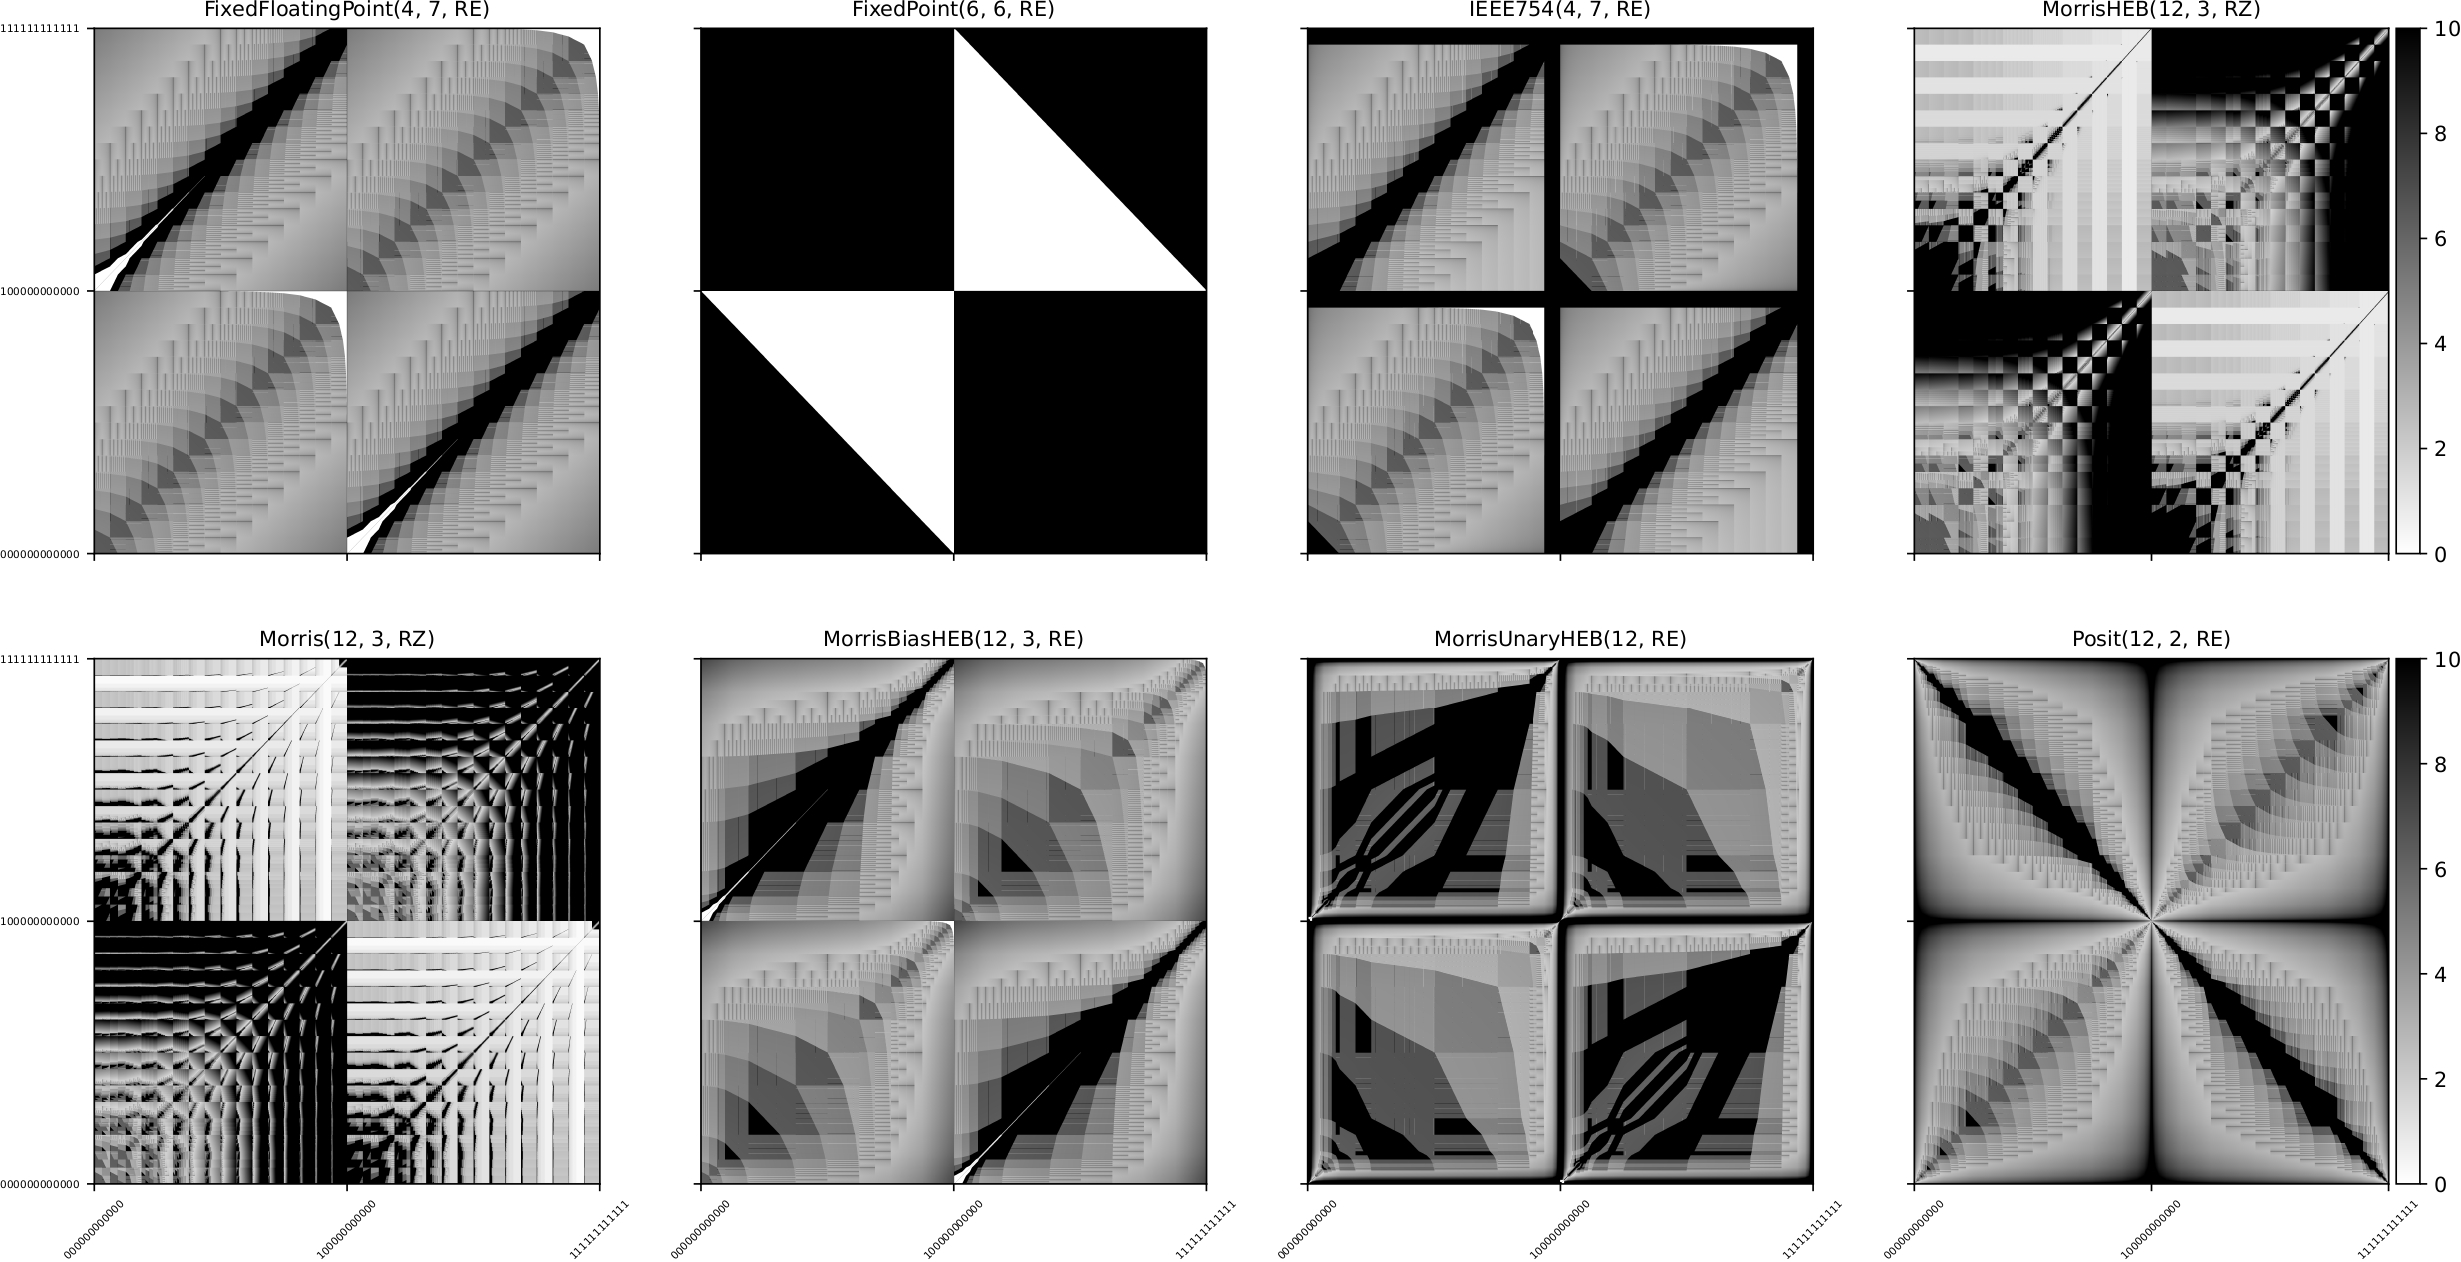
\includegraphics[width=\textwidth]{media/add.jpg}
\end{figure}

\end{frame}


\begin{frame}
    \frametitle{Multiplication}
    \begin{figure}[tp]
    \includegraphics[width=\textwidth]{media/mul.jpg}
    \end{figure}
\end{frame}

\begin{frame}
    \frametitle{Exam Questiion}
    Template: Given the hexadecimal string $0x\text{hex}$, what is the value of the number in the X NRS (number representation system)?
    
    Example: Given the binary string $0x5A$, what is the value of the number in the Morris Hidden Exponent Bit with Bias G (8, 2) representation?
\end{frame}
